% !TeX root = ../main.tex
\section{问题一：确定性电价下的日前购电优化}
\subsection{模型概述}
根据0{:}00时已知的分时电价、负荷需求和光伏预测功率，本文建立单日确定性储能调度模型(LP)。
模型以各时段的外网购电量、储能充放电量、储电量和弃光量为决策变量，以全天计划购电费用最小为目标，并考虑微网能量平衡、储能状态转移、储电量边界、充放电功率限制及首尾储电量相等等约束。
求解模型后，可得到144个时段的计划购电量、储能充放电量和储电量变化，并进一步汇总六个四小时时段的充放电总量，以及全天购电量和购电费用。

\subsection{输入数据特征分析}
根据上文划分的144个时段数据，可以绘制出小区负荷、光伏预测功率、净负荷与分时电价的日内变化曲线。第 \(t\) 个时段对应的时刻为
\begin{equation}
    \tau_t=t\Delta t,
    \qquad
    \Delta t=\frac{1}{6}\,\mathrm{h},
    \qquad
    t=1,2,\ldots,144
    \label{eq:q1_time_axis}
\end{equation}

设 \(P_t^{\mathrm{L}}\) 和 \(P_t^{\mathrm{PV}}\) 分别为该时段的小区负荷功率和光伏预测功率，则净负荷为
\begin{equation}
    P_t^{\mathrm{net}}
    =
    P_t^{\mathrm{L}}-P_t^{\mathrm{PV}}
    \label{eq:q1_net_load}
\end{equation}

为方便比较与展示，绘图时我们将负荷、光伏和净负荷功率统一换算为 \(\mathrm{MW}\)，电价仍以元/\(\mathrm{kWh}\) 表示。
由图可见，中午光伏出力高于小区负荷，表明此时存在富余光伏。晚间光伏出力下降，而负荷和电价处于较高水平。
因此，我们初步判断可利用储能吸收中午的富余光伏，并在晚间释放，以减少高价时段的外网购电量。
\begin{figure}[htbp]
    \centering
    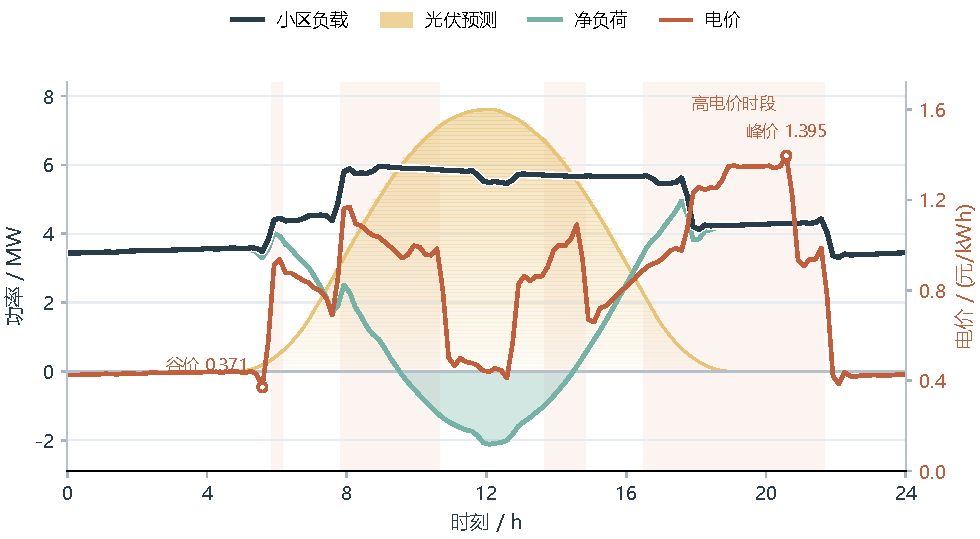
\includegraphics[width=0.85\textwidth]
    {../All_Code/Q1/Results/Pictures/q1_fig1_timeseries.pdf}
    \caption{问题一负荷、光伏预测、净负荷与电价的日内变化}
    \label{fig:q1_timeseries}
\end{figure}

\subsection{符号与变量说明}
除电价和效率参数外，后续模型中的负荷、光伏、购电、充放电及储电量均以 \(\mathrm{kWh}\) 为单位。
问题一使用的主要符号如下表所示。

\begin{table}[htbp]
    \centering
    \label{tab:q1_symbols}
    \begin{tabularx}{0.88\textwidth}
    {@{}>{\centering\arraybackslash}p{0.22\textwidth}
    >{\centering\arraybackslash}X@{}}
        \toprule
        符号 & 含义 \\
        \midrule
        \(t\) & 时段编号，\(t=1,2,\ldots,T\) \\
        \(\pi_t\) & 第 \(t\) 时段的外网购电价格 \\
        \(L_t\) & 第 \(t\) 时段的小区负荷电量 \\
        \(G_t\) & 第 \(t\) 时段的光伏预测发电量 \\
        \(x_t\) & 第 \(t\) 时段的计划购电量 \\
        \(c_t\) & 第 \(t\) 时段由交流母线送入储能的充电量 \\
        \(r_t\) & 第 \(t\) 时段由储能释放到交流母线的放电量 \\
        \(w_t\) & 第 \(t\) 时段未被利用的光伏电量 \\
        \(s_t\) & 第 \(t\) 时段结束时的储电量 \\
        \(\eta_c,\eta_r\) & 储能的充电效率和放电效率 \\
        \(S_{\min},S_{\max}\) & 储电量运行下限和上限 \\
        \(S_0\) & 储能在 \(0{:}00\) 时的初始储电量 \\
        \bottomrule
    \end{tabularx}
    \vspace{0.4em}
  \caption{问题一符号说明}
\end{table}

\subsection{模型建立}

\subsubsection{决策变量与目标函数}
以外网购电、储能充放电、弃光及储电状态作为调度对象，分别记为 \(x_t\)、\(c_t\)、\(r_t\)、\(w_t\) 和 \(s_t\)。
各时段的负荷电量 \(L_t\)、光伏预测发电量 \(G_t\) 与电价 \(\pi_t\) 由附件1给定。

问题一的目标是在满足负荷需求和储能运行约束的条件下，使全天计划购电费用最低。
第$t$时段的购电费用等于电价$\pi_t$乘以购电量$x_t$，全天计划购电费用为各时段费用之和。因此第一阶段目标为：
\begin{equation}
    C_1^{*}
    =
    \min \sum_{t=1}^{T}\pi_t x_t
    \label{eq:q1_stage1}
\end{equation}
充放电量不直接计入目标函数。储能运行产生的能量损耗通过状态递推方程体现，并最终转化为额外的购电需求。

\subsubsection{约束条件}

\begin{itemize}[label=\textbullet]

    \item \textbf{电量平衡约束}

    为保证供需严格平衡，每个时段的外网购电、光伏利用和储能放电共同满足负荷与充电需求，因此有
    \begin{equation}
        x_t+G_t-w_t+r_t=L_t+c_t,
        \qquad t=1,2,\ldots,T
        \label{eq:q1_balance}
    \end{equation}
    其中，\(G_t-w_t\) 为实际利用的光伏电量，\(w_t\) 为未被负荷或储能吸收的光伏电量。
    引入弃光变量后，所有电量都有明确去向，同时可以统计光伏消纳情况。

\item \textbf{储能状态转移约束}

  根据附录1，充电效率和放电效率均取 \(0.9\)。充电过程中，输入电量中只有 \(\eta_c c_t\) 会实际存入储能。放电过程中，若需向交流母线输出 \(r_t\) 电量，储能内部需要消耗 \(r_t/\eta_r\)。因此，储电量的状态转移方程为
  \begin{equation}
      s_t
      =
      s_{t-1}
      +\eta_c c_t
      -\frac{r_t}{\eta_r},
      \qquad
      \eta_c=\eta_r=0.9,
      \qquad
      t=1,2,\ldots,T
      \label{eq:q1_soc}
  \end{equation}

  例如，向储能输入 \(100\,\mathrm{kWh}\) 时，储电量实际增加 \(90\,\mathrm{kWh}\)。储能向交流母线输出 \(100\,\mathrm{kWh}\) 时，其内部电量减少约 \(111.11\,\mathrm{kWh}\)。
    \item \textbf{运行边界约束}

    储能最大充放电功率为 \(5000\,\mathrm{kW}\)，对应每个10分钟时段的最大充放电量为
    \begin{equation}
        q_{\max}
        =5000\times\frac{1}{6}
        =833.333\,\mathrm{kWh}
        \label{eq:q1_qmax}
    \end{equation}
    结合储电量范围、充放电能力及变量非负性，各时段满足
    \begin{equation}
    \begin{aligned}
        1200&\leq s_t\leq10800,\\
        0&\leq c_t\leq q_{\max},\\
        0&\leq r_t\leq q_{\max},\\
        x_t&\geq0,\\
        0&\leq w_t\leq G_t,
    \end{aligned}
    \qquad t=1,2,\ldots,T
    \label{eq:q1_bounds}
    \end{equation}
    为保证所得调度方案能够按日重复执行，根据题目对首尾储电量的要求，设置日循环边界
    \begin{equation}
        s_0=s_T=6000\,\mathrm{kWh}
        \label{eq:q1_terminal}
    \end{equation}
\end{itemize}

\subsubsection{第二阶段优化模型}

第一阶段得到最低购电费用 \(C_1^*\)的最优解可能不唯一，其中部分方案存在不必要的充放电循环。
为此，第二阶段保留原模型的全部约束，增加费用上限，并把目标换为储能总吞吐量：
\begin{equation}
    \min \sum_{t=1}^{T}\left(c_t+r_t\right)
    \label{eq:q1_stage2}
\end{equation}
同时满足：
\begin{equation}
    \sum_{t=1}^{T}\pi_t x_t
    \leq C_1^*+\varepsilon,
    \qquad
    \varepsilon=10^{-4}\,\mathrm{元}
    \label{eq:q1_cost_tolerance}
\end{equation}
由此得到购电费用最优且充放电过程更简洁的调度方案。

\subsection{模型求解}

\subsubsection{线性规划转换}

上述模型的目标函数及约束条件均为线性关系，本文将其转化为标准线性规划。按照购电量、充电量、放电量、弃光量和储电量的顺序，将决策变量排列为
\begin{equation}
    \boldsymbol{z}
    =
    \left(
    x_1,\ldots,x_T,
    c_1,\ldots,c_T,
    r_1,\ldots,r_T,
    w_1,\ldots,w_T,
    s_1,\ldots,s_T
    \right)^{\mathrm T}
    \label{eq:q1_variable_vector}
\end{equation}
由于 \(T=144\)，模型共包含 \(720\) 个连续决策变量。

将附件1中的电价、负荷电量和光伏预测发电量代入模型，整理为
\begin{equation}
\begin{aligned}
    \min_{\boldsymbol z}\quad
    &\boldsymbol f_1^{\mathrm T}\boldsymbol z,\\
    \mathrm{s.t.}\quad
    &\boldsymbol A_{\mathrm{eq}}\boldsymbol z
    =\boldsymbol b_{\mathrm{eq}},\\
    &\boldsymbol l\leq\boldsymbol z\leq\boldsymbol u
\end{aligned}
\label{eq:q1_standard_lp}
\end{equation}
其中，目标向量 \(\boldsymbol f_1\) 的前144个元素为各时段电价，其余元素为零。
\(\boldsymbol A_{\mathrm{eq}}\) 由144条电量平衡约束、144条储能状态转移约束和1条末端储电量约束构成，共289行。
右端向量 \(\boldsymbol b_{\mathrm{eq}}\) 由净负荷电量 \(L_t-G_t\) 和初末储电量条件确定。
各变量的运行范围则通过上下界 \(\boldsymbol l,\boldsymbol u\) 设置。

储能状态以 \(s_0=6000\,\mathrm{kWh}\) 为起点，通过相邻时段的状态转移连接全天调度，并以 \(s_T=6000\,\mathrm{kWh}\) 作为终端条件。
据此构造的线性规划同时求解各时段的购电、充放电、弃光及储电量。
\subsubsection{两阶段求解}

第一阶段调用 HiGHS 求解购电费用最小化模型，同时得到各时段的购电量、充放电量、弃光量和储电量。最低购电费用为
\begin{equation}
    C_1^\ast
    =
    35126.948589\,\mathrm{元}
    \label{eq:q1_stage1_result}
\end{equation}

随后保留原有约束，加入式 \eqref{eq:q1_cost_tolerance} 的费用上限，并将目标函数改为储能总充放电量最小，再次调用 HiGHS 求解。
第二阶段得到最终调度方案
\[
\left\{
x_t^\ast,c_t^\ast,r_t^\ast,w_t^\ast,s_t^\ast
\right\}_{t=1}^{144}
\]
其中，\(s_t^\ast\) 是在电量平衡和储能状态转移约束下与其他变量同时求得的逐时段储电量。

\subsubsection{求解结果汇总}

根据第二阶段的逐时段最优解，计算全天购电量、购电费用、充电量、放电量和总吞吐量
\begin{equation}
\begin{aligned}
    E_{\mathrm{buy}}&=\sum_{t=1}^{T}x_t^\ast, &
    C_2&=\sum_{t=1}^{T}\pi_t x_t^\ast,\\
    E_{\mathrm{ch}}&=\sum_{t=1}^{T}c_t^\ast, &
    E_{\mathrm{dis}}&=\sum_{t=1}^{T}r_t^\ast,\\
    E_{\mathrm{through}}
    &=E_{\mathrm{ch}}+E_{\mathrm{dis}}
\end{aligned}
\label{eq:q1_result_summary}
\end{equation}
相应结果为
\[
\begin{aligned}
    E_{\mathrm{buy}}&=59482.699\,\mathrm{kWh},\\
    C_2&=35126.948689\,\mathrm{元},\\
    E_{\mathrm{ch}}&=20740.665\,\mathrm{kWh},\\
    E_{\mathrm{dis}}&=16799.939\,\mathrm{kWh},\\
    E_{\mathrm{through}}&=37540.603\,\mathrm{kWh}
\end{aligned}
\]
第二阶段购电费用与第一阶段最低费用仅相差 \(10^{-4}\,\mathrm{元}\)。

模型直接求得的是储电量 \(s_t^\ast\)。为描述储能荷电状态，将其换算为
\begin{equation}
    \mathrm{SOC}_t
    =
    \frac{s_t^\ast}{12000}\times100\%.
    \label{eq:q1_soc_conversion}
\end{equation}
求解结果中，储电量在 \(1200\,\mathrm{kWh}\) 至 \(10800\,\mathrm{kWh}\) 之间变化，对应 SOC 的变化范围为 \(10\%\) 至 \(90\%\)。日初和日末储电量均为 \(6000\,\mathrm{kWh}\)，对应 SOC 均为 \(50\%\)。

最后，将144个时段的 \(x_t^\ast\) 作为计划购电量输出，并将每24个连续时段的 \(c_t^\ast\) 和 \(r_t^\ast\) 分别求和，得到题目要求的六个四小时时段充放电总量。